%\documentclass{standalone}
\documentclass{standalone}
\usepackage{tikz}
\usetikzlibrary{shapes,arrows,positioning,decorations.pathreplacing,decorations.markings}
\usepackage{amsmath,bm,times}
\usepackage{lmodern}
\usepackage[utf8]{inputenc}
\usepackage[T1]{fontenc}
\usepackage{graphicx}
\usepackage{multimedia}
\renewcommand{\familydefault}{\sfdefault}

%\usepackage{fontspec}
%\setmainfont[BoldFont={Roboto-Bold.ttf},
%ItalicFont={Roboto-LightItalic.ttf},
%BoldItalicFont={Roboto-BoldItalic.ttf}
%]{Roboto-Light.ttf}
%\setmainfont{Roboto}

\begin{document}

\pagestyle{empty}

\pgfdeclarelayer{background}
\pgfdeclarelayer{foreground}
\pgfsetlayers{background,main,foreground}


\definecolor{rpi}{RGB}{0,134,59}
\definecolor{ard}{RGB}{16,162,174}
\definecolor{sand}{RGB}{242,240,218}
\definecolor{romi}{RGB}{53,168,100}


\tikzstyle{human}=[draw,fill=sand, text width=8em, text centered, minimum height = 4em]
\tikzstyle{refine}=[draw,fill=sand, text width=5em, text centered, minimum height = 4em]



\begin{tikzpicture}
\node (human) [human] {Small set of noisy labels};
\path (human.south)+(0,-1.5) node (labels) {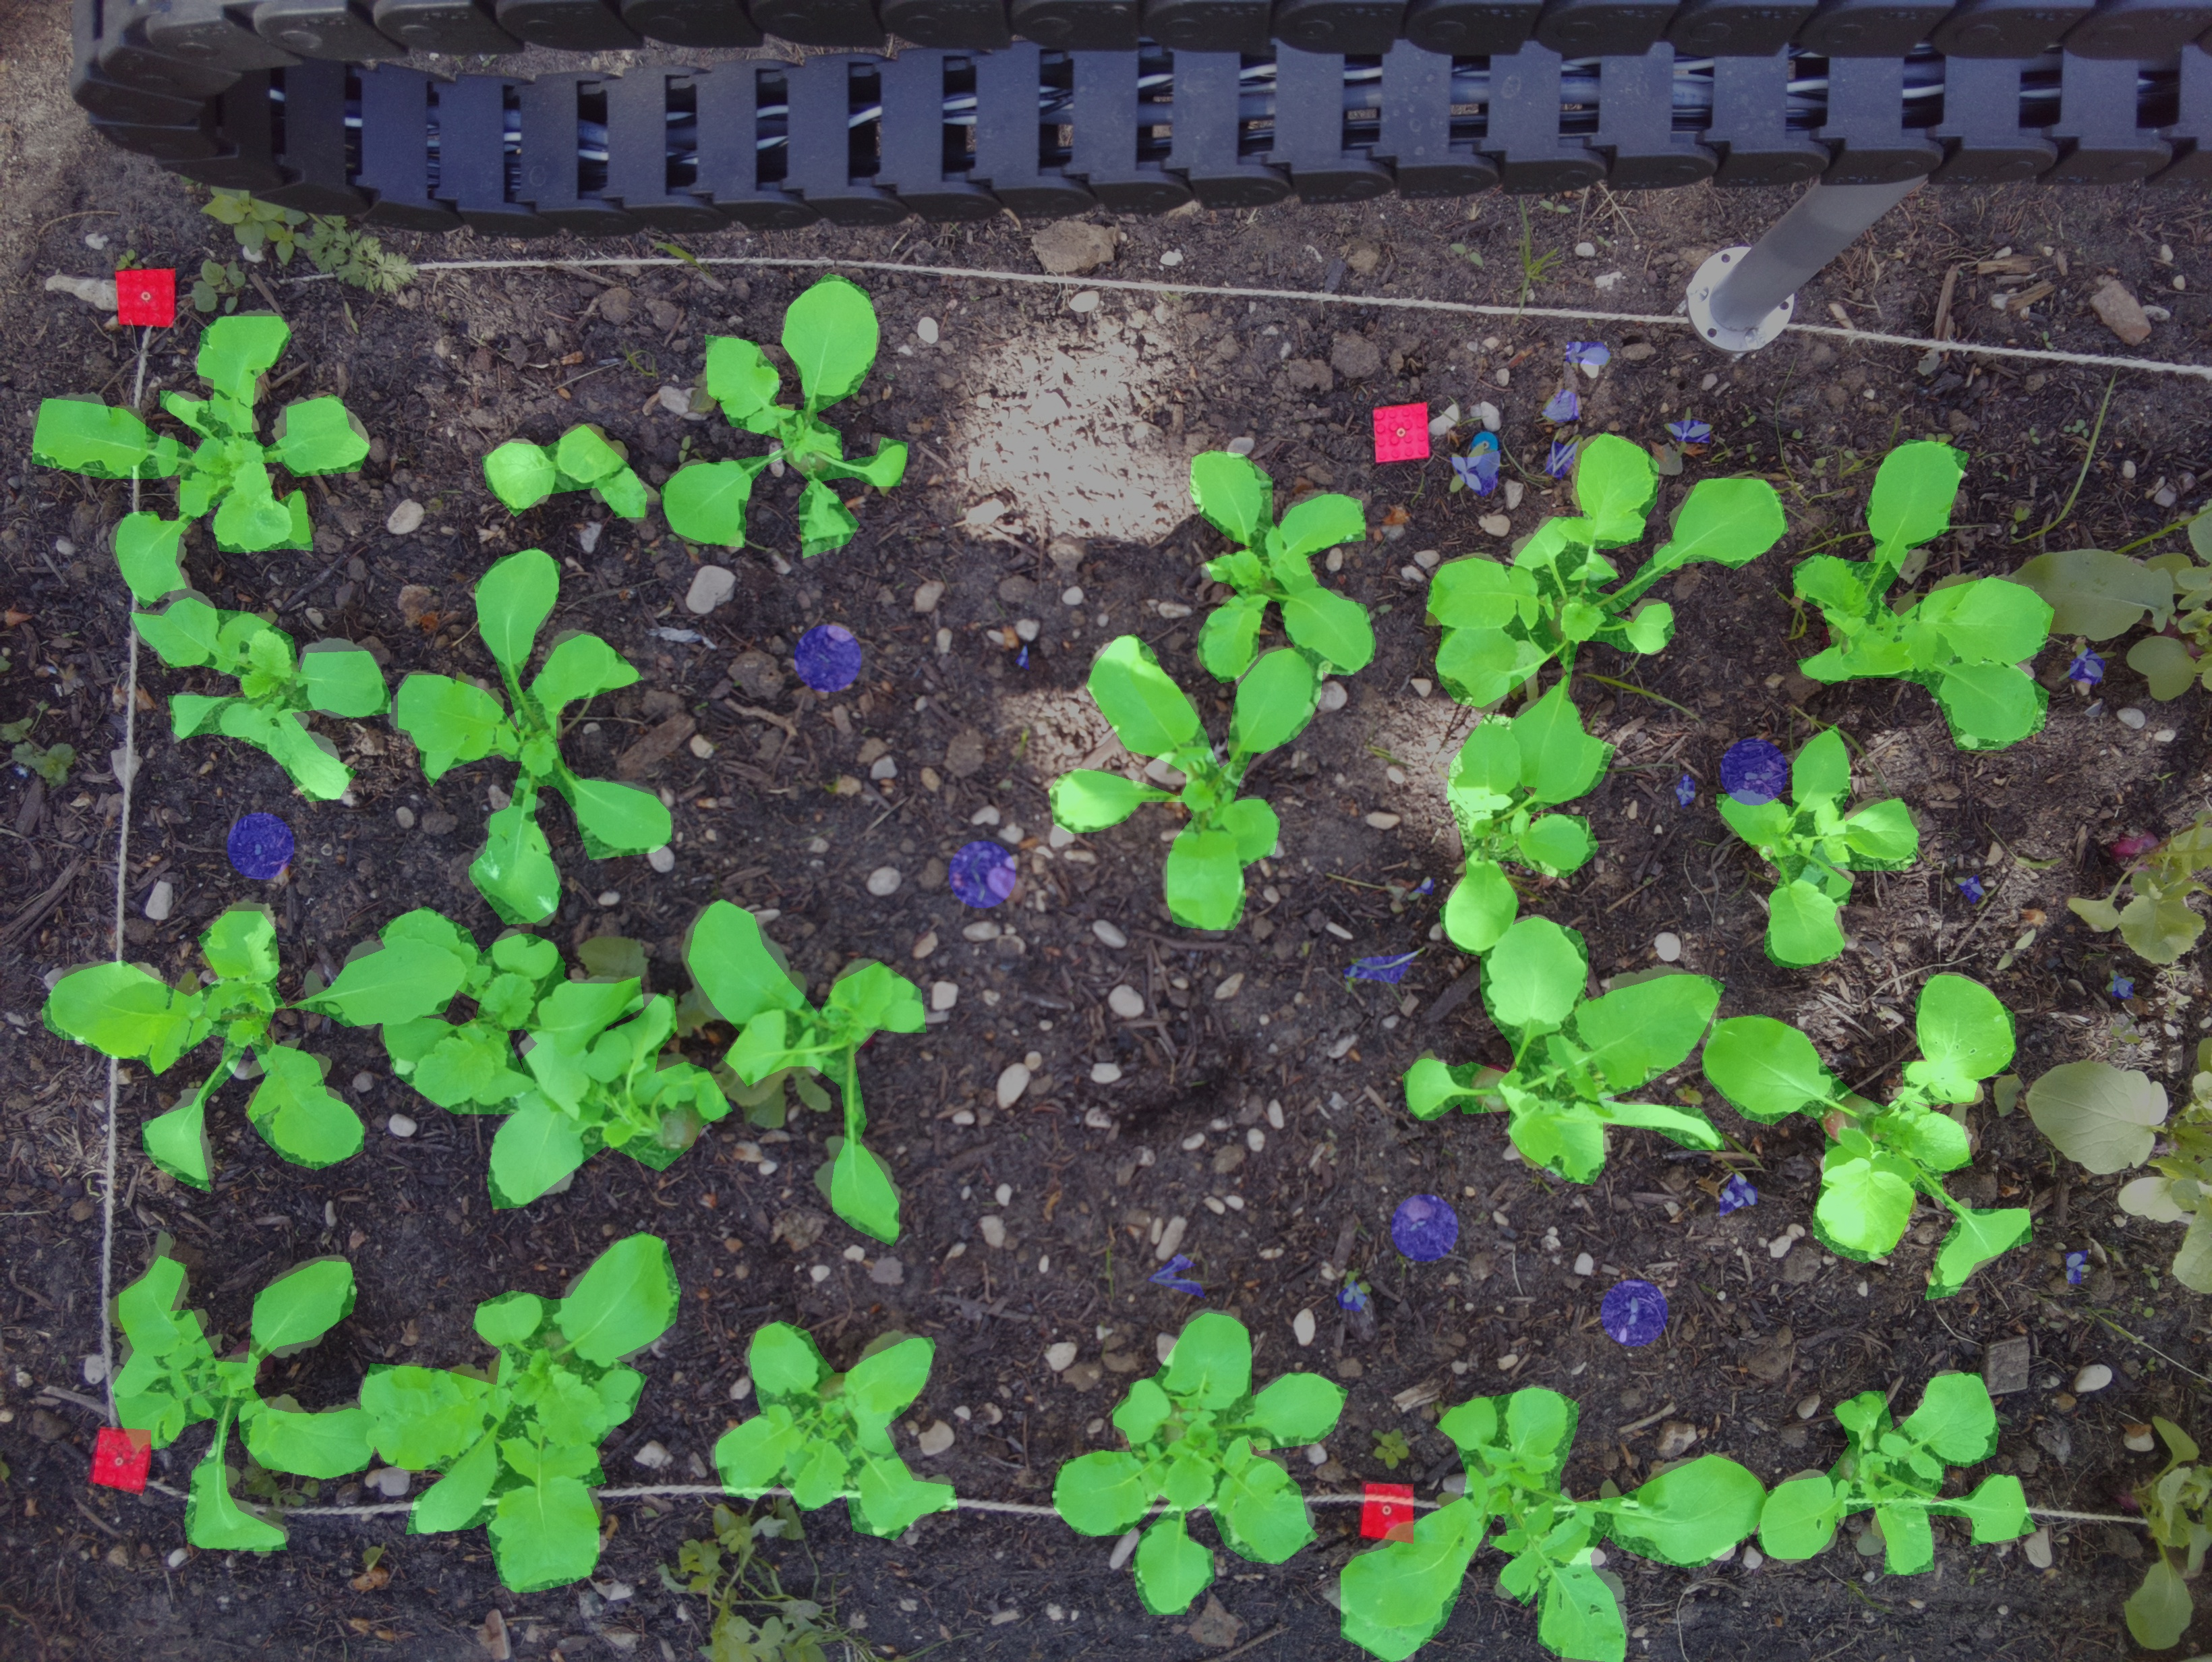
\includegraphics[width=10em]{annotations}};
\path (human.east)+(3,0) node (ref) [refine] {Small set of clean data}; 
\path (ref.south)+(0,-1.5) node (refvid) {\movie[label=mavideo,width=10em,autostart]{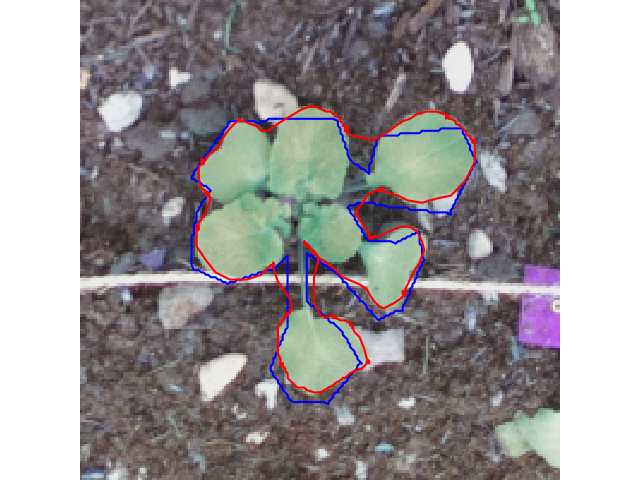
\includegraphics[width=10em]{100}}{ref_short.webm}\hyperlinkmovie[play,pause]{mavideo}{}};
\path (ref.east)+(3,0) node (clean) [refine] {Large set of (almost) clean data}; 
\path (clean.south)+(0,-1.5) node (refvid) {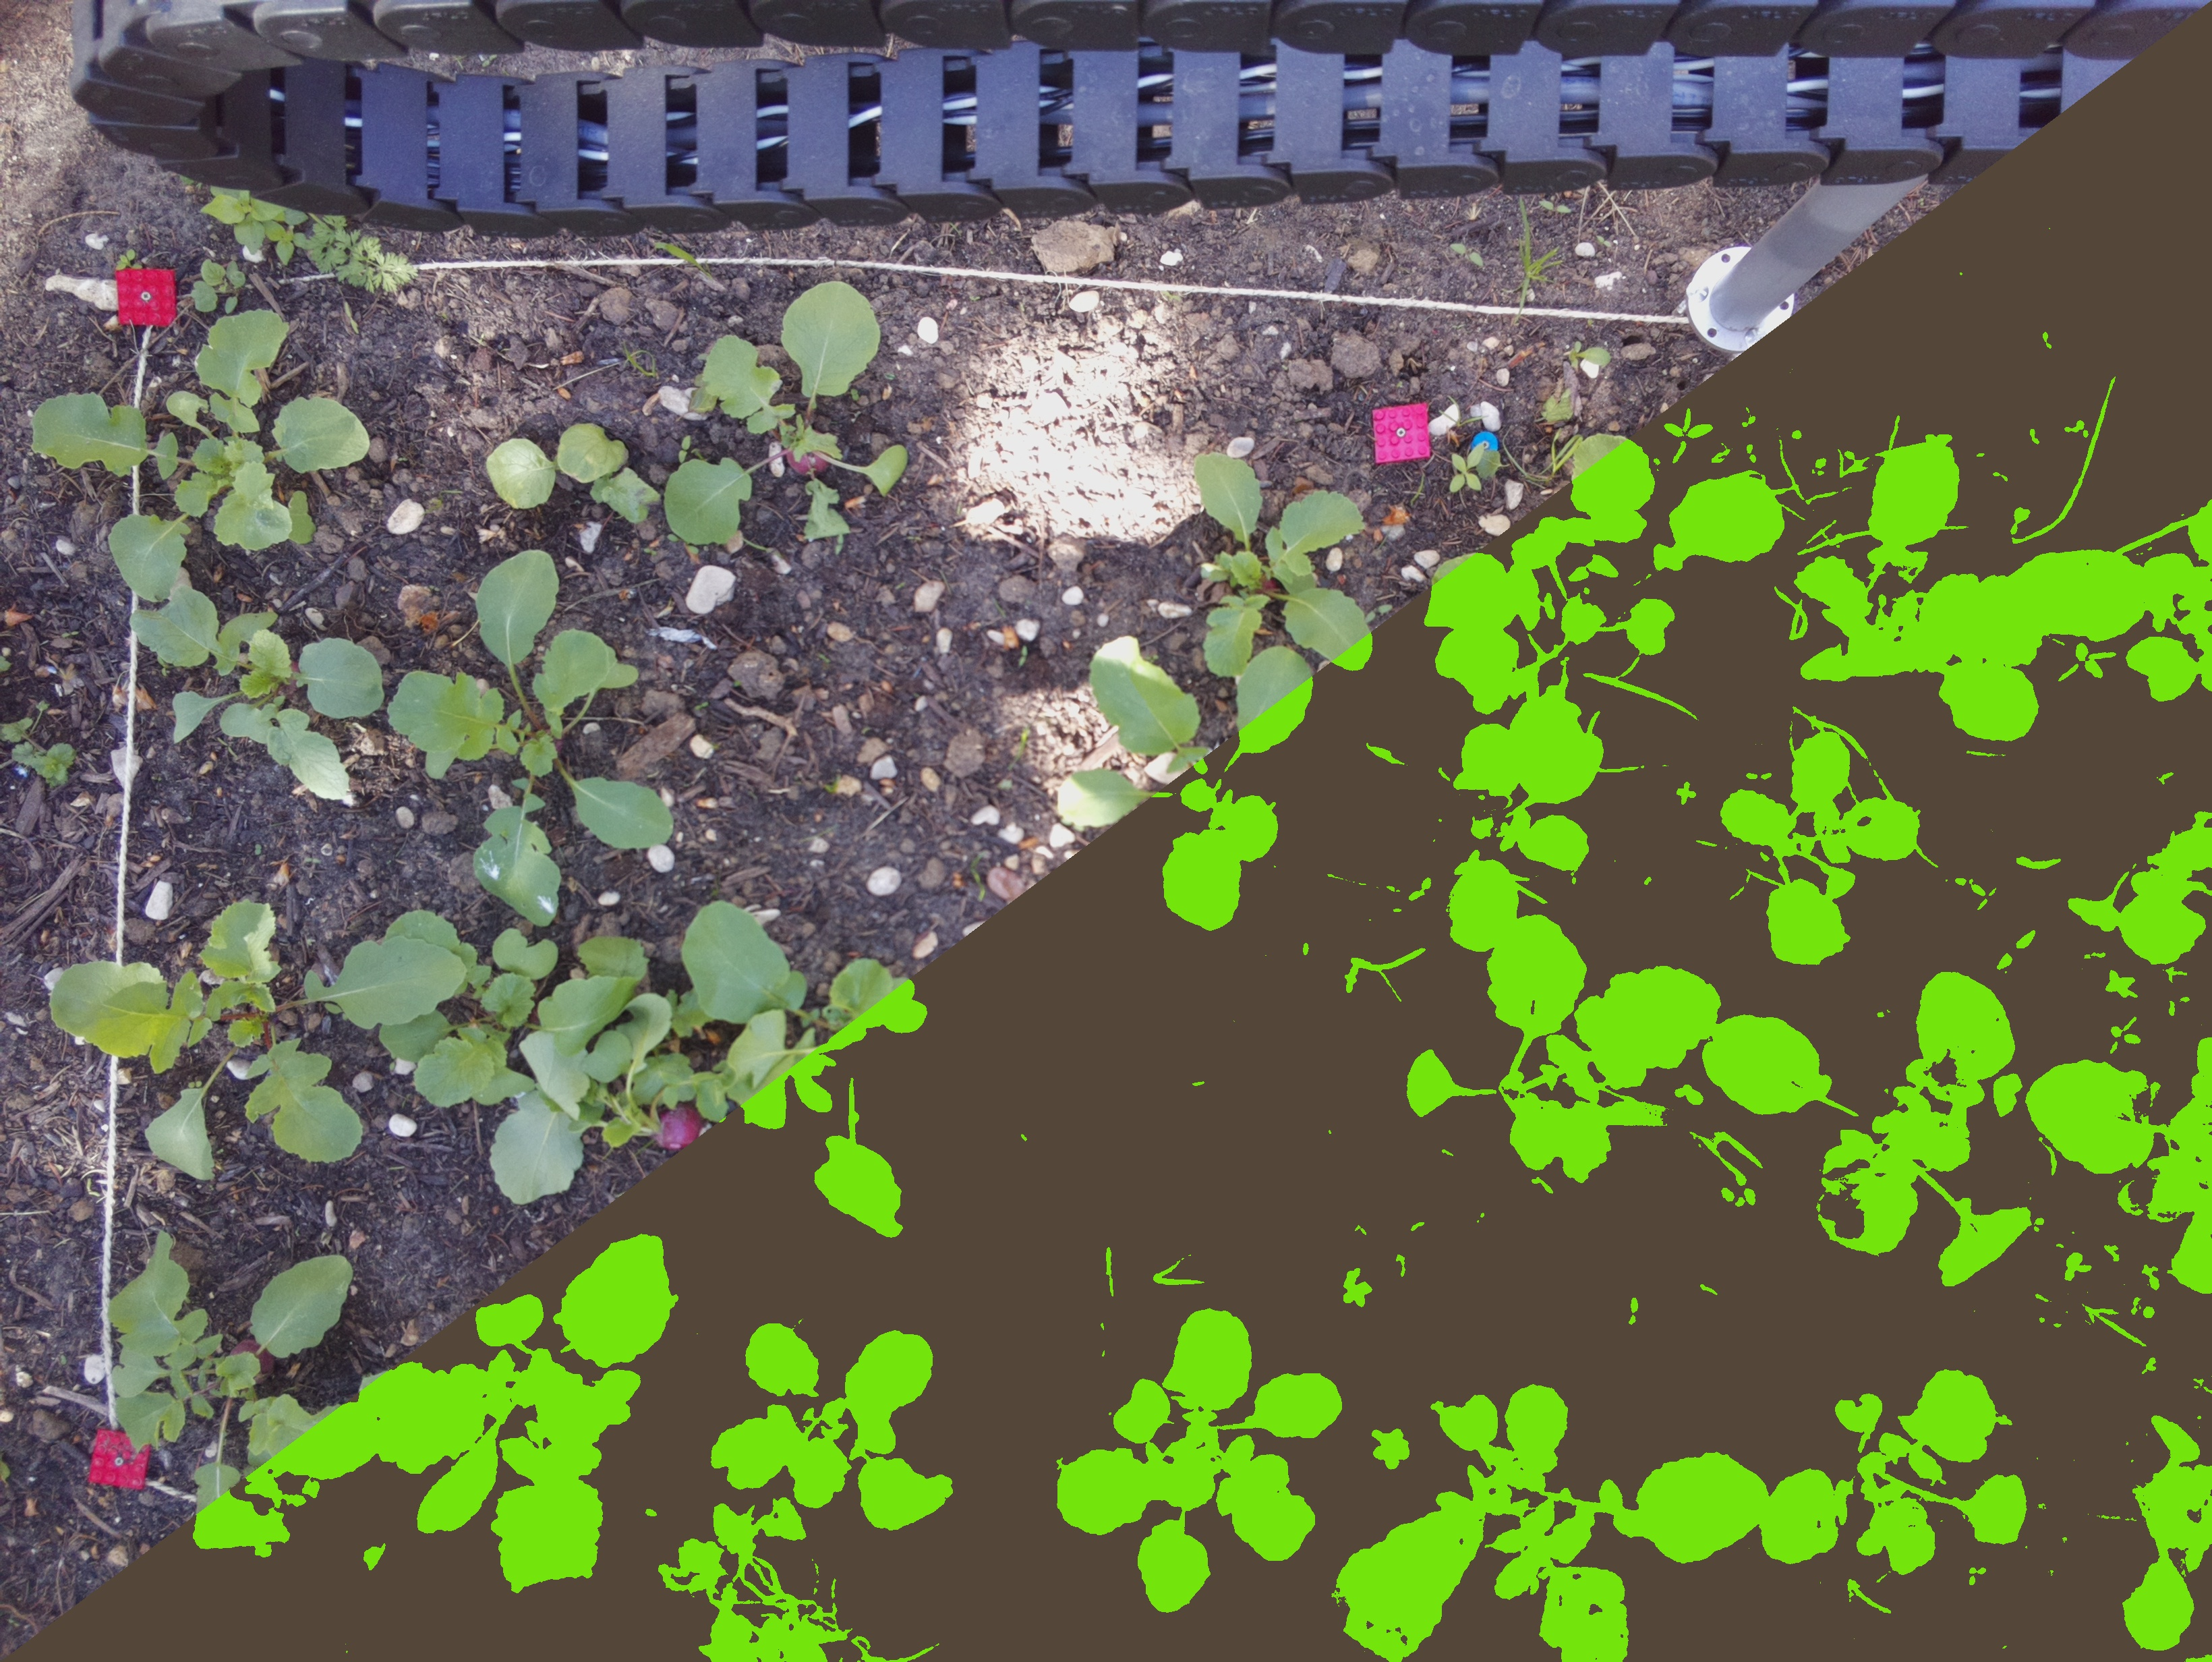
\includegraphics[width=10em]{mixMask_05_12}};

\draw [->] (human) -- node[above] {Active} node[below] {contours} (ref) -- node[above] {Classifier} node[below] {\tiny \it e.g.,SVM} (clean);

\end{tikzpicture}
\end{document}